\chapter{Icecube Neutrino Observatory}

Why is icecube so big, bit science smalltalk here?
The IceCube Neutrino observatory is the largest neutrino detector on earth.
Located on the south pole and shown schematically in figure \ref{fig:icecube}.

\begin{figure}
    \centering
    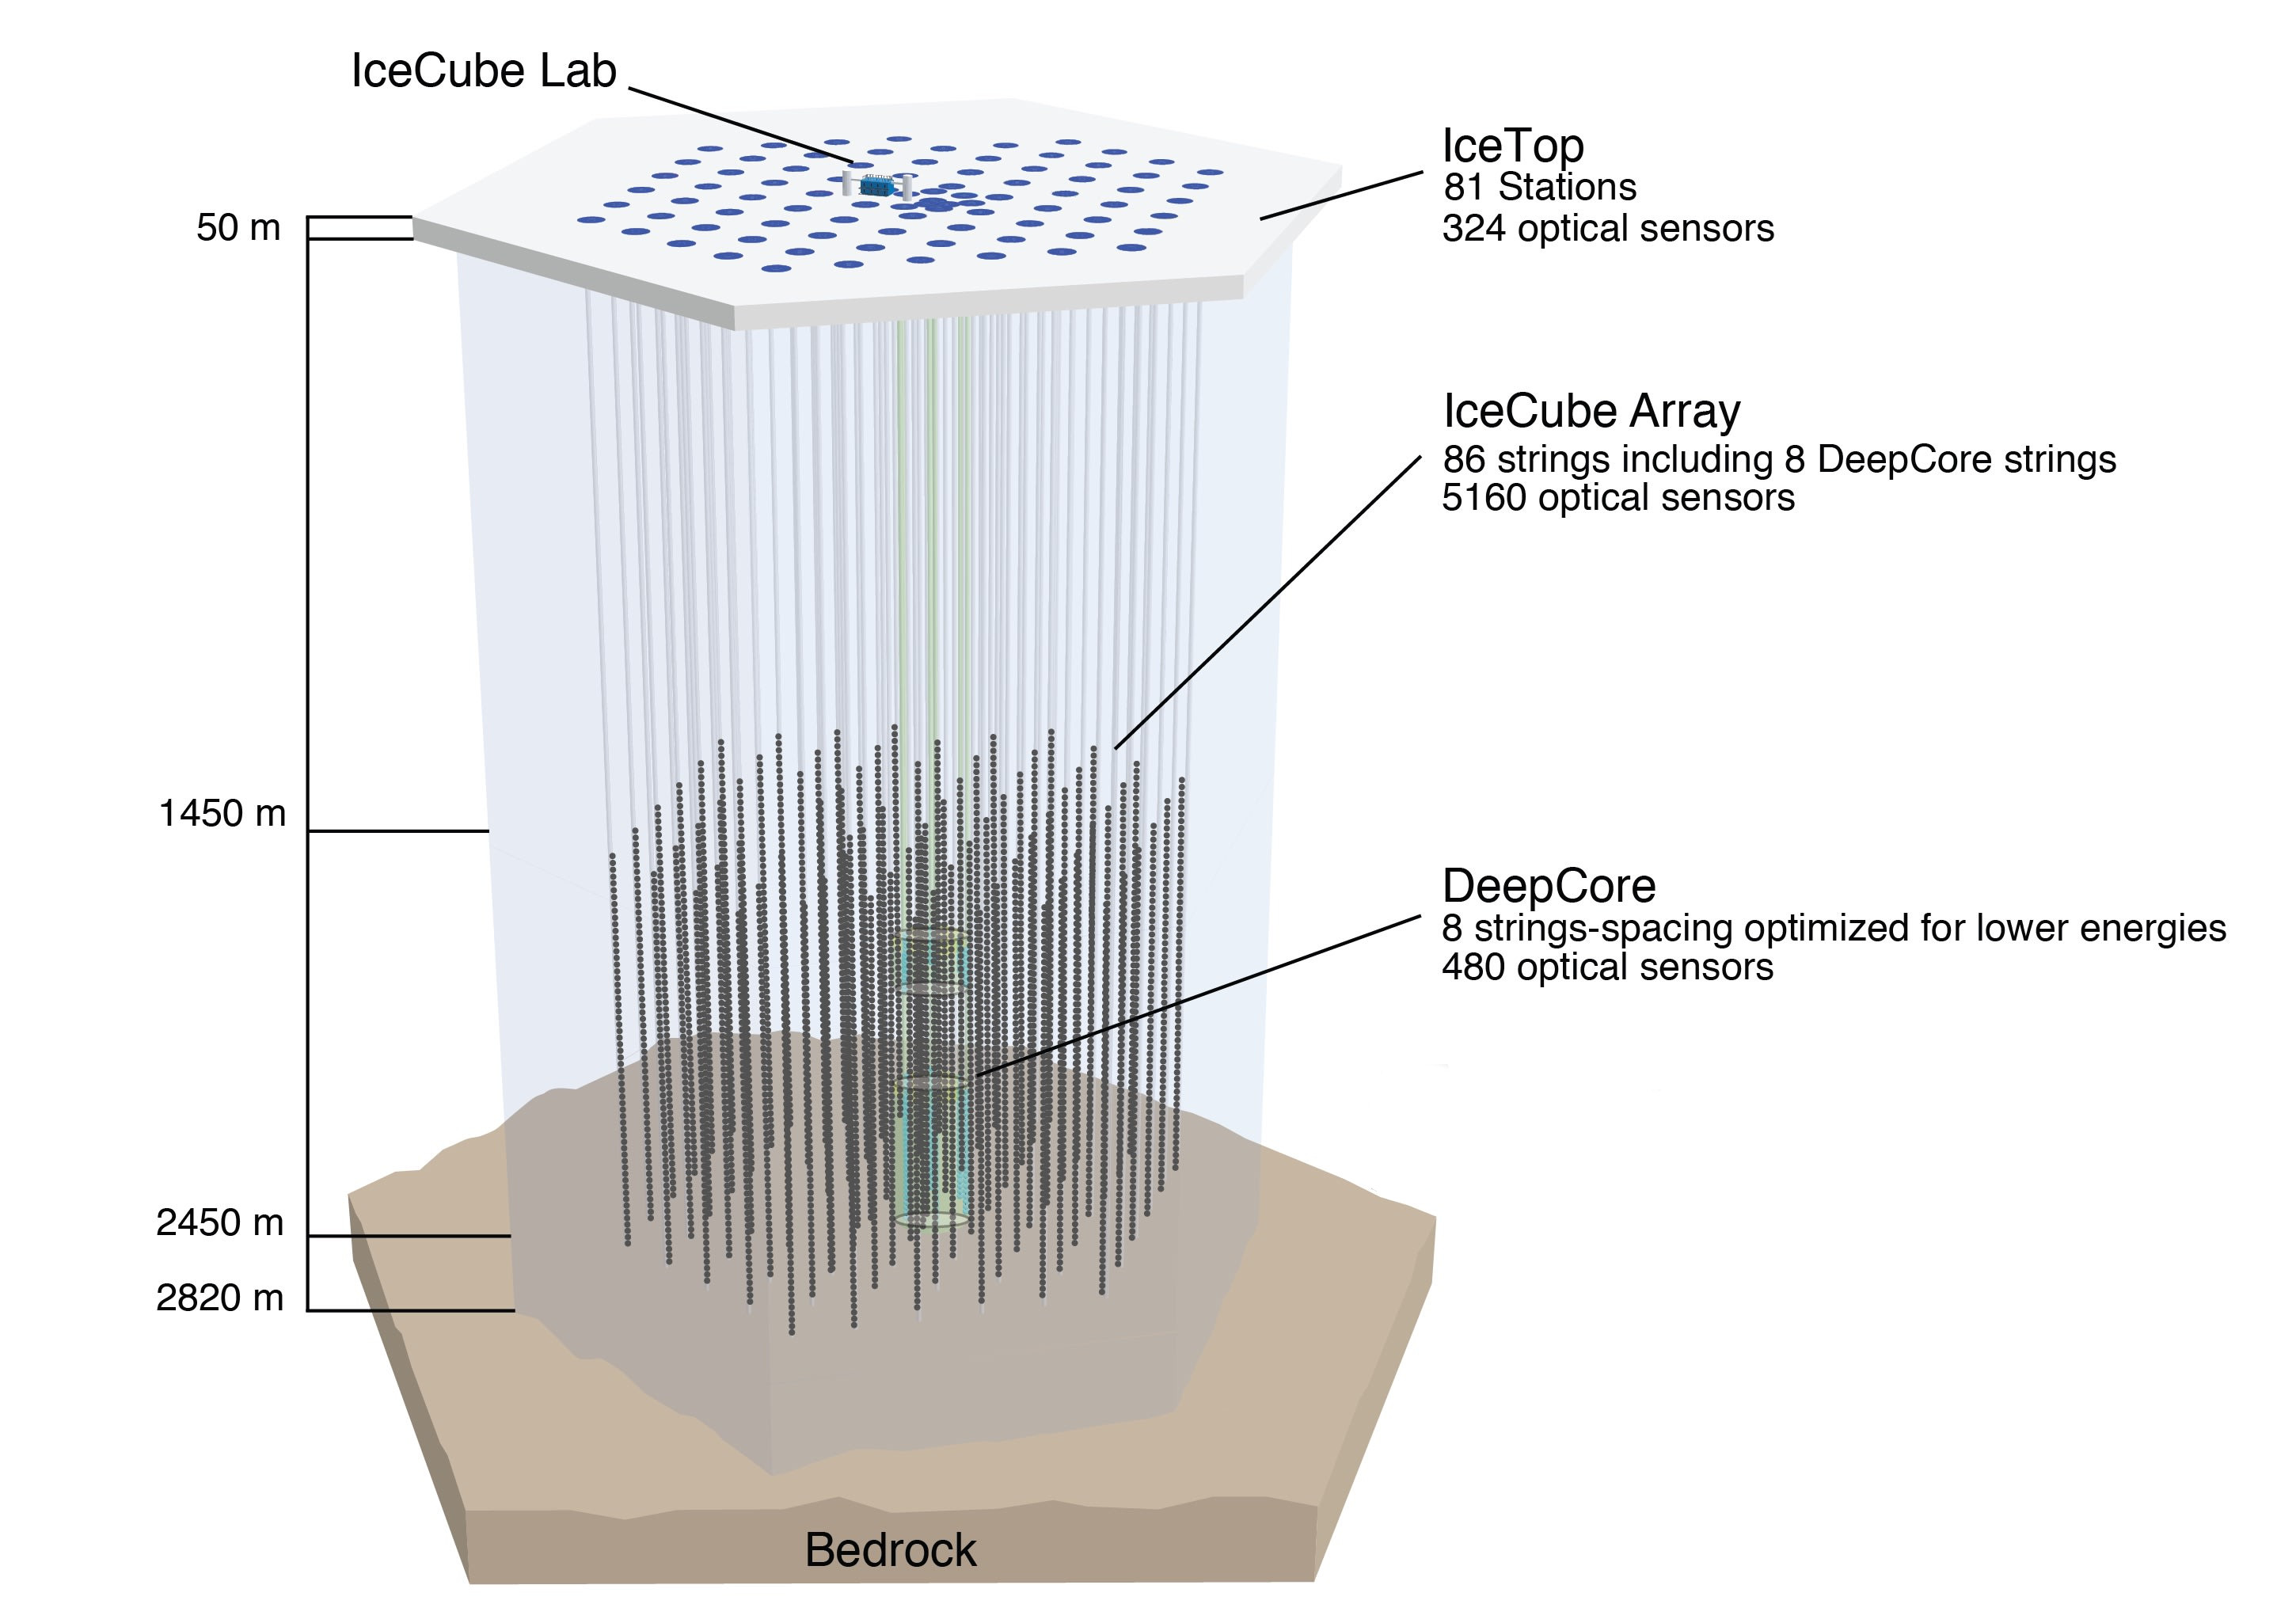
\includegraphics[width=10cm]{Plots/01_7_icecube/IceCube-Array.jpg}
    \caption{\cite{icecube_website}.}
    \label{fig:icecube}
\end{figure}

Construction started 2004 and took 7 years to its completion in 2010.
The detector volume of IceCube covers about 1 cubic kilometer of clear antarctic ice.
86 holes were drilled in the ice to let down cables with 60 digital optical modules (DOMs) each.
The detecion volume, or the position of the first DOM respectively, starts at a depth of about 1450 meters and ends in a depth of about 2450 meters.
Mention IceTop and DeepCore?
IceCube detects about 275 million cosmic rays every day.
bit more about doms


\section{Detection Principle}
cherenkov something something\\
show interaction\\
make a figure to cherenkov\\

\section{Tracks and Cascades}

To perform a point source search, two properties of the detector signatures of the muons are of particular importance: the direction and the energy.
It is therefore important to distinguish between two types of events, tracks and cascades.
Tracks pass through the detector but do not deposit all their energy in the detector volume.
This means that the direction of the event can be reconstructed very well.
The signature left by such an event can be seen in figure \ref{fig:track}.
However, since the total energy is not deposited in the detector volume, the reconstruction of the energy is generally not optimal.
\begin{figure}
    \centering
    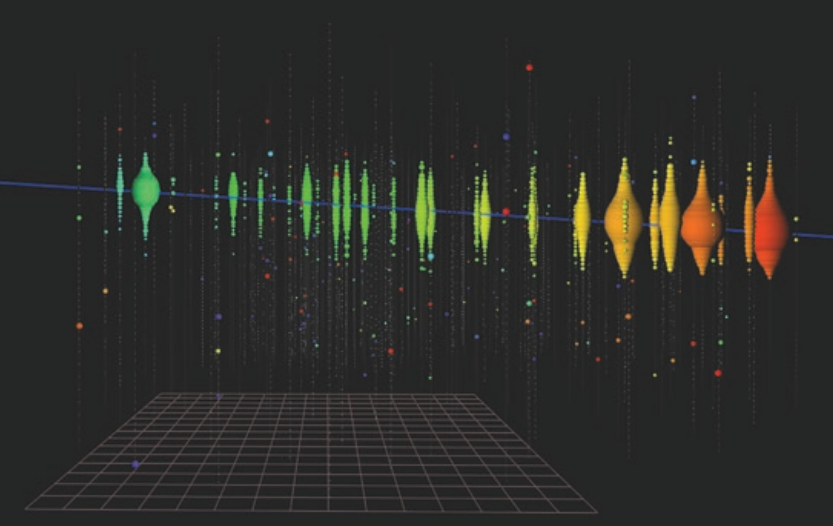
\includegraphics[width=10cm]{Plots/01_7_icecube/track.png}
    \caption{tracklike event signature in the detectorvolume. The deposited energy is represented by the size of the spheres, the time of arrival by the colour (blue earlier, red later). The small glow of individual modules is unfiltered noise \cite{spiering}.}
    \label{fig:track}
\end{figure}
Cascades, on the other hand, deposit their entire energy in the detector volume, which means that the energy can be determined quite accurately.
Due to the shape of the cascade event, however, the original direction is very difficult to reconstruct.
Such an event can be seen in figure \ref{fig:cascade}.
Generally, the magnitude of the event's energy is the main statistical indicator of whether an event is astrophysical in origin, but the exact reconstruction of the event's direction is very important for a point source search.
Therefore, a dataset from tracks is usually used.
However, due to their high energy, cascade events can be used as a source catalogue, but this is not the case in this thesis.
\begin{figure}
    \centering
    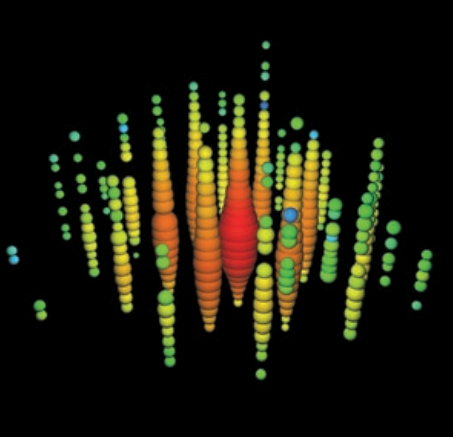
\includegraphics[width=10cm]{Plots/01_7_icecube/cascade.png}
    \caption{The filtered cascade event named \textit{Ernie} with a reconstructed energy of $\SI{1.04}{\peta\electronvolt}$. The deposited energy is represented by the size of the spheres, the time of arrival by the colour (blue earlier, red later) \cite{spiering}.}
    \label{fig:cascade}
\end{figure}
